\noindent
Graph processing is a critical component in a broad range of applications ranging from  social network analysis, medical diagnostics, and drug interaction studies.  Given the vast size of these graphs with billions of edges and vertices, graph algorithms stress memory and scaling capabilities of computing systems. In this proposal we treat graph algorithms as linear algebraic problem formulations, where graphs are represented as adjacency matrices.  The evolving duality between graph algorithms and their equivalent matrix operations forms a solid basis for designing computing systems that can efficiently manipulate matrix operations.  For example, there are well known linear algebraic problem formulations for graph algorithms such as breadth first search, strongly connected components, shortest path, stress centrality, betweenness centrality,  sub-graph detection and so on.  These algorithms demand a diverse range of matrix manipulations, including matrix multiplication, Kronecker product,  matrix decomposition, inner and outer products, matrix inversion, matrix transpose and Eigen value computation.  Supporting such a broad range of operations on extremely large matrices is the first challenge that will be tackled in this proposal. 

%An equally daunting challenge is the representation of large graphs as adjacency matrices in memory.
Given the diversity of application domains where graph analytics may be used, the structure of graphs may also be varied. To improve storage and bandwidth efficiency sparse graphs may be stored in  (double) compressed sparse row (CSR) and column (CSC) formats. But sparse graph representations also worsen irregular access patterns to memory. Some graphs may exhibit power law distributions where only a few vertices contribute to most edges in the graph. Such disparity leads to significant load imbalances in computations.  Efficiently handling both sparse and dense matrices with varying degrees of connectivity is the second challenge tackled in this proposal. 
 
Finally, scaling the execution of linear algebraic manipulations, through parallelization, while mitigating Amdahl's bottleneck is the last challenge that this proposal tackles. Parallel execution of matrix operations can be mapped to various distributed computing paradigms, such as Mapreduce, Pregel and Parallel-R. For instance, many PGAS (partitioned global address space) approaches distribute equal number of vertices across nodes (equal number of rows from the adjacency matrix). 
But when vertex degrees exhibit power law distribution it  is extremely difficult to balance the load across computational nodes. Launching a  new iteration of the computation  requires the previous iteration to complete, thereby forcing a barrier synchronization across various threads. In the presence of load imbalances such synchronizations curtail scaling. 

These observations lead to the main research thrusts of this proposal, as described below. To guide the discussion of the proposed research we present an overview of the system architecture that we will design and build. The system will rely on processing-in-memory architecture, but appropriately adopted for matrix manipulations used in graph processing. Figure~\ref{fig:arch} present the overview of the architecture . The basic building block of the GAMA (graph acceleration through matrix abstraction) system is a GAMA corelet, which is a 16-wide SIMD pipeline that is optimized by vector multiply-accumulate operations. Each corelet is provisioned with \emph{Elastic} L1 cache.  32 corelets are placed on a single die and share a single large L2 cache designed using eDRAM. The L2 cache is then backed up by 4X8GB DiRAM4 memory modules. DiRAM4 is a die-stacked DRAM die that is provided by Tezzaron (one of our service providers in this project). The 32 corelets are 2.5D stacked with DiRAM4. This entire package is called a GAMA tile. We will integrate 16 GAMA tiles to create the whole GAMA accelerator system. 16 GAMA tiles are interconnected  using our custom-designed 1Tbps inter-tile interface. The GAMA system is interfaced with IBM Power8-based host system using OpenCAPI interface. 

At each layer of the above design we propose several innovative ideas. At the corelet layer we propose to design specialized address mapping engines that translate the sparse matrix indices to generate the row/column index of matrix elements based on the underlying sparse matrix format. While the 32 GAMA corelets can do MIMD computations they can  be dynamically reconfigured to execute a single instruction across a very wide vector range when accesses are highly sequential.  The elastic  cache attached to each corelet is architected to support both dense/sequential and sparse/random accesses to a matrix. The elastic cache is a low-overhead cache organization that supports variable width cache lines to improve cache usage efficiency.  
 The unique aspect of DiRAM4 memory, compared to other competing memories such as high bandwidth memory, is that each DiRAM4 die supports more channels per die, but uses narrow width channels. Such a design is well suited for graph workloads that need narrow width memory level parallelism. The narrow width channels can be reconfigured to create a single wide width channel to support dense matrices. The memory layer itself is made semantically aware of the matrix structure and its preferred lay out and access patterns in memory. The semantic awareness comes from application provided hints that are conveyed to the memory controller through APIs. Since graphs that are spread over multiple tiles demand high bandwidth inter-tile access. High-bandwidth links  posing power, thermal, and signal integrity challenges.  We tackle this challenge with various charge-based and injection-locking techniques for high-speed links. The scalability of parallel graph algorithms will be improved by enabling barrier elision hardware that can be used by the application developer to tradeoff accuracy with latency. We provide an in-depth visibility to software to monitor changes to the graph structure and take action to deal with potential load imbalances.  
\begin{figure}
\center
%\vspace{-8ex}
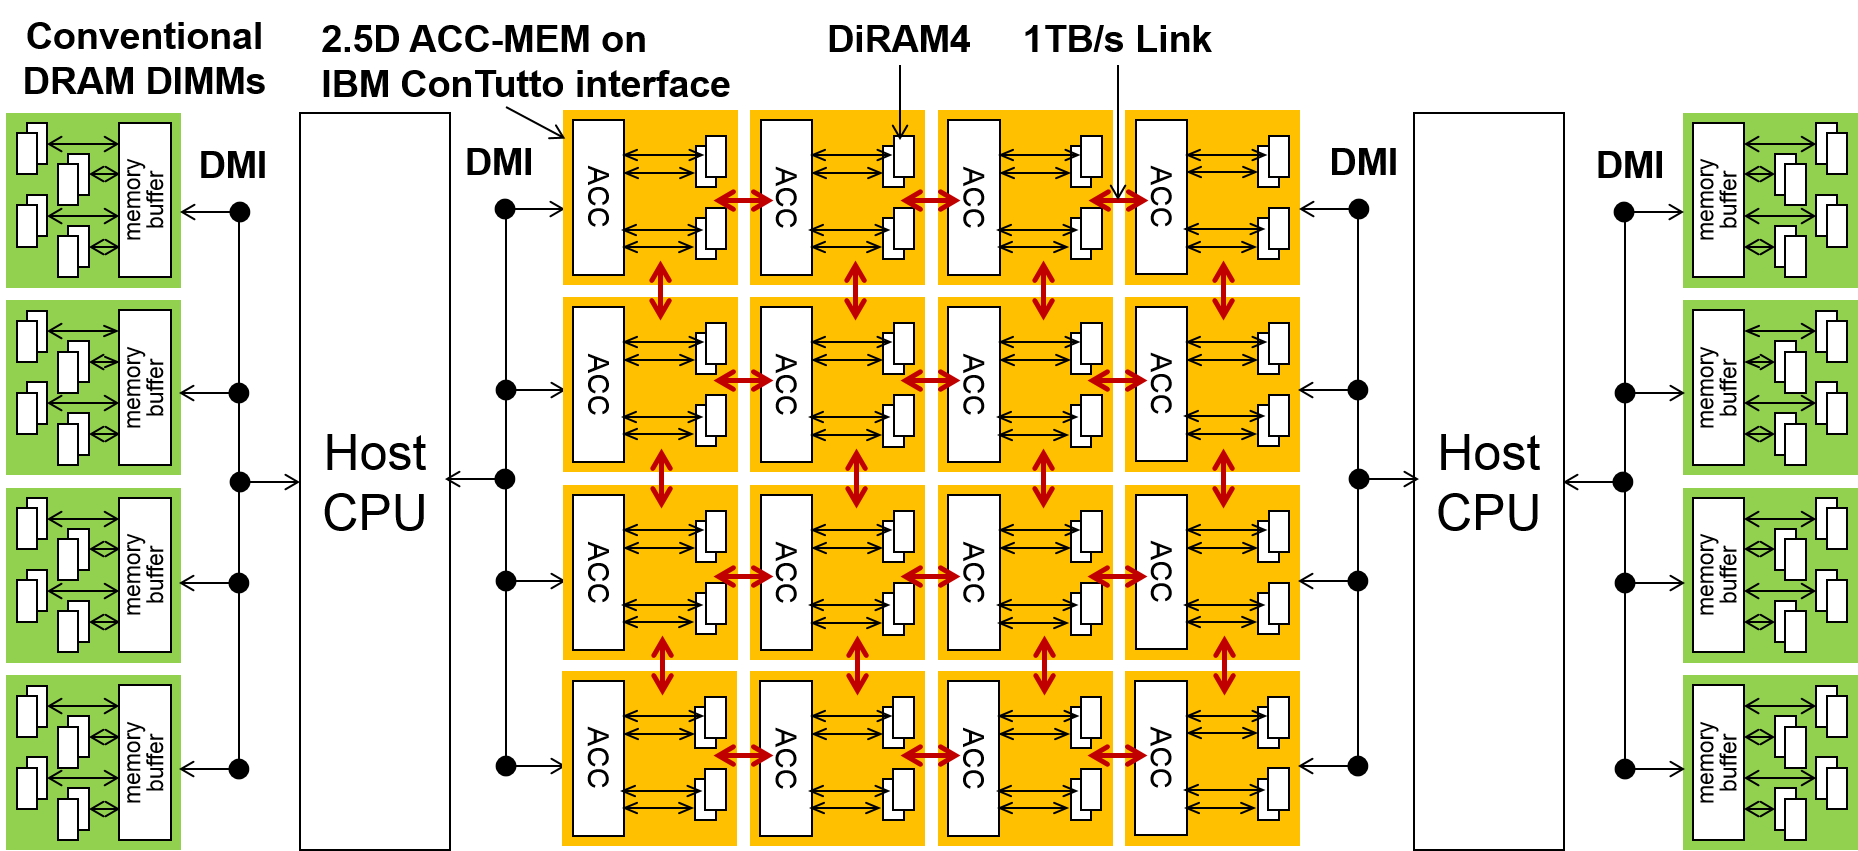
\includegraphics[width=1.0\linewidth]{fig/arch.png}
\caption{GAMA System Architecture}
\label{fig:arch}
\end{figure}


